\documentclass[a4paper, 12pt]{article}
\usepackage[left=2cm,
            right=2cm,
            top=2cm,
            bottom=2cm,
            bindingoffset=0cm]{geometry}
% \usepackage{array}
% \usepackage[indent=0pt]{parskip}
\usepackage{hyphsubst}
\usepackage{setspace}
% \singlespacing
\usepackage{enumitem}
\setenumerate{noitemsep,topsep=0ex}

\usepackage{hyperref}
% \usepackage{float}
% \usepackage{graphicx}
% \graphicspath{ {./images/} }
% \usepackage{subfig}
% \usepackage{enumerate}
\usepackage[normalem]{ulem} % underlining
% \usepackage{booktabs} % tables
% \PassOptionsToPackage{table}{xcolor}% coloring tables

% LANGUAGE + FONT
		    
\usepackage[english]{babel}
\usepackage{csquotes}

% \usepackage{natbib}
% \renewcommand{\bibsection}{~\\\textbf{References}}
% \bibpunct[: ]{[}{]}{;}{a}{}{,}
% \bibliographystyle{rusnat}

\usepackage[style=authoryear, backend=biber]{biblatex}
\addbibresource{../../ref.bib}
\addbibresource{ref.bib}

\usepackage{fontspec}  
\setmainfont{Garamond}

% DRAWING

\usepackage{tikz}
\usepackage{tikz-qtree}
\usetikzlibrary{shapes.geometric}
\usetikzlibrary{trees,arrows}
\usetikzlibrary{positioning}

% LINGUISTICS 

%\usepackage{gb4e}
\usepackage{expex}
\lingset{aboveglftskip=0ex, belowglpreambleskip=0ex, belowexskip=2ex, aboveexskip=1ex, interpartskip=0ex}

\gathertags
\usepackage[glossaries]{leipzig}
\newleipzig{cmpr}{cmpr}{Comparative}
\newleipzig{sprl}{sprl}{Superlative}
\newleipzig{indef}{indef}{Indefinite}
% \makeglossaries

\usepackage{stmaryrd}

% MATH
\usepackage{amssymb}

\begin{document}
\begin{sloppypar}

% -------------------------- текстиктекстиктекстик -----------------------------
{\large \textbf{\cite{abels2012linearasymmetrieslca}. Linear Assymmetries and the LCA}}
\\~

\textbf{Background.} Kayne’s \parencite*{kayne1994antisymmetrysyntax} seminal work, addressing assymmetries found in syntax, proposes Linear Correspondence Axiom (LCA), which suggests that linear order of constituents corresponds to asymmetrical c-command relation. Asymmetrical c-command is defined as (\nextx). By LCA, if a non-terminal X asymmetrically c-commands a non-terminal Y, then all terminals X dominates precede all terminals Y dominates.

\ex
    X c-commands Y iff X and Y are categories and X excludes Y and every category that dominates X dominates Y.
\xe

It is widely assumed \parencite[e.g.][]{cinque2005derivinggreenberguniversal} that LCA entails an X'-like phrase template, which \textcite{abels2012linearasymmetrieslca} refer to as spec-head-comp hypothesis (SHCH). It states that branching is binary; that every phrase has a unique head that determines the category of all dominating nodes; that a head combines with no more than two phrases (one comp, then one spec) and is linearized between them, in order spec~---~head~---~comp.

% \begin{enumerate}
%     \item Every syntactic projection has a unique head whose category is inherited by all nodes within its projection that dominate it (endocentricity).
%     \item No head combines with more than two phrasal categories within its projection (single specifier/adjunct restriction).
%     \item If a head combines with two phrases within its projection, it is linearized as higher~phrase~---~head~---~lower phrase (spec-head-comp order).
%     \item Projections are binary branching.
% \end{enumerate}

\textbf{SHCH does not follow from LCA.} \textcite{abels2012linearasymmetrieslca} show that none of these properties follow from LCA. The problem is that LCA does not provide a theory of node labeling, which it must tentatively borrow from X'-theory \parencite[cf.][414]{chomsky1995}. First of all, there is nothing in LCA itself that requires nodes to inherit their category from the head and rules out structures like (\nextx).

\ex<>
    [\textsubscript{PP} [\textsubscript{V} v] [\textsubscript{NP} [\textsubscript{N} n]]]
\xe

Second, if more than two levels of projection are allowed, multiple specifiers can be adjoined under different levels (e.g. \nextx). Even if the number of levels is restricted to two, adjunction to a head \parencite[17]{kayne1994antisymmetrysyntax} is allowed for phrases on a similar basis. It follows that head-final linearization is available for LCA.

% \textbf{Endocentricity.} Heads in \parencite{kayne1994antisymmetrysyntax} are defined as "nonterminal[s] that dominate no other nonterminal". This definition, indeed, forbids structures with multiple heads and with no heads.\footnote{Two sister heads c-command each other, and the terminals are unordered. Two sister nonheads c-command each other's daughters, and the terminals are ordered contradictorily.} However, since labeling is unrestricted, it is not required that higher nodes inherit the head's category: e.g. [\textsubscript{PP} [\textsubscript{V} v] [\textsubscript{NP} [\textsubscript{N} n]]]

% \textbf{Single spec and comp.} If there are multiple specifiers under a single category X, they c-command each other's daughters, leading to contradictory linear order. However, if more than two levels of projection are allowed, multiple specifiers can be adjoined under different levels (e.g. \nextx). U does not c-command Y here since V'' does not dominate Y. Thus, even if we only allow heads to project, two specifiers for a single head are still not banned.

\ex<>\\
    \begin{tikzpicture}[sibling distance=5ex]
        \Tree [.V$''$ [.X [.Y y ] ]
                  [.V$''$ [.V$'$ [.U [.W w ]]
                                 [.V$'$ [.V v ]
                                       [.S [.T t ]]]]]]
    \end{tikzpicture}
\xe

% \textbf{Spec-head-comp order.} Even if we restrict the number of bar levels, generating head-final structures is still possible via adjunction to the head \parencite[17]{kayne1994antisymmetrysyntax}. A phrase can be adjoined to the head in a way similar to (\lastx).

% \ex<>
%     [\textsubscript{XP} [\textsubscript{YP} [\textsubscript{Y} y]] [\textsubscript{XP} [\textsubscript{X} [\textsubscript{ZP} [\textsubscript{Z} z]] [\textsubscript{X} x]]]]
% \xe

Finally, ternary branching is not ruled out, e.g., in cases like (\nextx), where a phrase (a subject) and a head (an adverb) are adjoined to a phrase.

\ex<>\\
    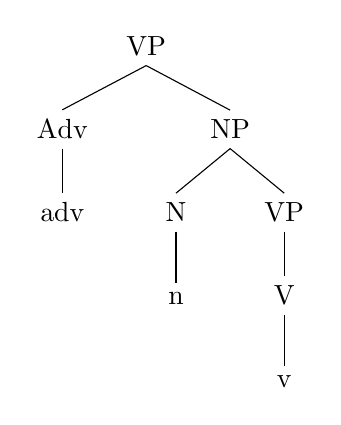
\begin{tikzpicture}[sibling distance=5ex]
        \Tree [.VP [.Adv adv ]
                   [.NP [.N n ]
                   [.VP [.V v ]]]]
    \end{tikzpicture}
\xe

\textbf{Predictive power.} Thus, SHCH does not follow from LCA and requires no less stipulation than a symmetrical theory of phrase structure. \textcite{abels2012linearasymmetrieslca} also show that it makes the same predictions about possible linear orders of constituents. What is worse, it also appeals to movement operations that contradict certain restrictions on movement, which are based on independent evidence. The most notable is antilocality \parencite[a.m.o.]{abels2003}: no complement can move to the specifier of its head. E.g., the complement of C is unextractable, since it must pass through Spec,CP (\nextx). However, movement of IP to Spec,CP would be required in SHCH for all complementizer-final structures. From there, extraction is thought to be possible, which leaves the data in (\nextx) unexplained.

\pex<>
    \a<> This book, I doubt that Mary has read.\trailingcitation{extraction out of Comp,CP}
    \a<> That Mary has read this book, I doubt.\trailingcitation{CP extraction}
    \a<> \ljudge*Mary has read this book, I doubt that.\trailingcitation{*Comp,CP extraction}
\xe

\textbf{Conclusion.} The requirement of stipulations and the lack of explanatory power makes LCA an unattractive theory. Linear ordering can be realized via ordering statements instead \parencite[e.g.][]{foxpes2005}, while hierarchical ordering of modifiers can be reduced to scope relations \Parencite[e.g.][]{nilsen2004}. Still, several linear assymmetries remain unexplained, such as the ban on rightward movement, but there is no reason to believe that those are better captured by LCA than by a symmetric syntactic theory.
\pagebreak

\textbf{Discussion.} The paper presents arguments, more or less novel, that the antisymmetry hypothesis is methodologically equivalent, but empirically weaker than symmetric approaches, and thus unattractive. It can be argued that, by deriving word orders through movement, LCA reduces syntactic variation to features, while a symmetric theory requires additional linear ordering tools; but it is shown that movement involved in local linearization in LCA obeys different rules than traditional movement, and that there are no empirical data in favor of their common nature.

The paper mentiones, but leaves unexplained many instances of the assymmetry of syntax, apart from Cinque's modifier orders. A number of such facts are provided a Kaynean explanation by \textcite{kayne2005} himself, but \textcite{tonoike2007japanesesymmetrysyntax} shows that these do not favor LCA even without \Citeauthor{abels2012linearasymmetrieslca}'s pedantry. Furthermore, a more recent discussion \parencite{zeijlstra2023} regarding the Final-over-Final Constraint \parencite{biberauer2014} undermines LCA's predictive power in the domain where it should strive. Overall, the tendency is that antisymmetry lacks not only theoretical, but empirical foundation, too.


% \bibliography{ref}
\printbibliography

\end{sloppypar}
\end{document}
